
\section{Function Class Implementation}
\label{c2:fc}

The commands used to control the controller itself and ot manage the Z-Wave network
are called 'function classes'. Most function classes used in the Sigma Designs
Serial API are used by the Z-Way lower layer function only but some of them 
are exposed to the Z-Wave Device API to allow user interactions and network management.

The Expert UI is an excellent reference for the Function Classes. All relevant functions 
can be monitored 'in action'. Hence the description of the network tab of the Expert 
UI is more or less a complete reference to the function classes needed in a UI implementation.

 
\begin{figure} 
\begin{center}
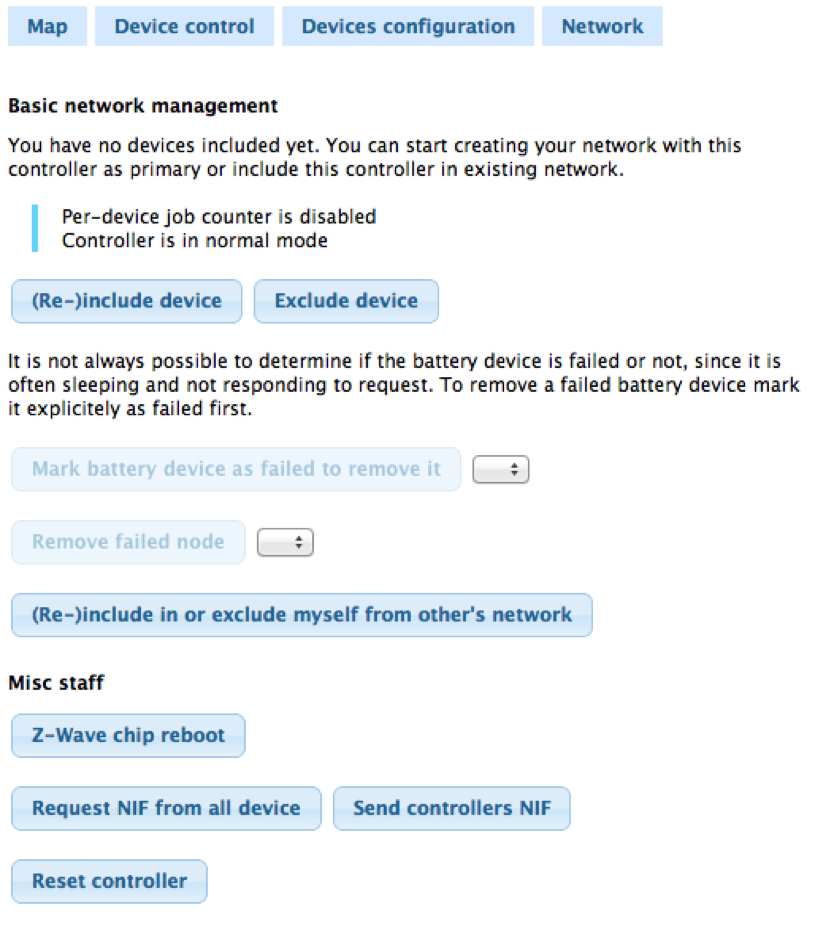
\includegraphics[scale=0.8]{pics/network1.png}
\caption{Expert UI Dialog for Networking functions}
\label{c1:network1} 
\end{center} \end{figure}

\subsection{Inclusion}

 You can include devices by pressing the 'Include Device' button. This turns the 
controller into an inclusion mode that allows including a device.  A status information 
line indicates this status. The inclusion of a device is typically confirmed with a 
triple press of a button of this particular device. However, please refer to the manual of 
this particular device for details how to include them into a Z-Wave network. The 
inclusion mode will time out after about 20 seconds or is aborted by pressing the 
'Stop Include' button.

If the network has a special controller with SIS function (Z-Way will try to activate 
such as function on default, hence this mode should always be active if the USB 
hardware used by Z-Way supports it) the inclusion of further devices can also be 
accomplished by using the include function of any portable remote control which 
is already included into the network.   A short explanation above the include button 
will inform about the ways devices can be included.

The Inclusion function is implemented using the function class 
{\bf AddNodeToNetwork(flag)} with flag=1 for starting the inclusion mode and 
flag=0 for stopping the  inclusion mode. Please refer to the chapter \ref{FunctionClasses} 
for details on how to use this function.


\subsection{Exclusion}

You can exclude devices by pressing the 'Exclude Device' button. This turns the controller 
into an exclusion mode that allows excluding a device. 
The exclusion of a device is typically confirmed with a triple press of a button of this 
particular device as well. However, please refer to the manual 
of this device for details how to exclude them into a Z-Wave network. The exclusion mode 
will time out after about 20 seconds or is aborted by pressing the 
'Stop Exclude' button.
It is possible to exclude all kind of devices regardless if they were included in the 
particular network of the excluding controller.

If a node is not longer in operation it can’t be excluded from the network since exclusion 
needs some confirmation from the device. Please use the 'Remove Failed Node' function 
in this case. 
Please make sure that only failed nodes are moved this way. Removed but still function 
nodes  - called phantom nodes – will harm the network stability.


The Exclusion function is implemented using the function class 
{\bf RemoveNodeToNetwork(flag)} with flag=1 for starting the exclusion mode and flag=0 
for stopping the 
exclusion mode. Please refer to the chapter \ref{FunctionClasses} for details on how to use this function.

\subsection{Mark Battery powered devices as failed}

This function allows marking battery-powered devices as failed. Only devices marked as 
failed can be excluded from the network without using the exclusion 
function. Typically multiple failed communications with a device result in this marking. 
Battery powered devices are recognized as sleeping in the controller 
and therefore all communication attempts with this device will be queued until a wakeup 
notification from this device is received. A faulty battery operated 
device will never send a wakeup notification and hence there is never a communication, 
which would result in a failed node status. Battery operated devices 
can therefore be manually marked as faulty.  Make sure to only mark  and subsequently 
remove  devices that are faulty or have disappeared. A device, which 
was removed with this operation but is still functioning may create malfunctions in the network.

This function is no Function class but sets the internal 'failed' variable of the device
object.

\subsection{Remove Failed Nodes}

Z-Way allows removing a node, if and only if this node was detected as failed by the 
Z-Wave transceiver. The network will recognize that communication with a device fails 
multiple times and the device can’t be reached using alternating routes either. 
The controller will then mark the device as 'failed' but will keep it in the current 
network configuration.  Any successful communication with the device will remove the 
failed mark. Only devices marked as failed can be removed using the 'Remove Failed Node' 
function.

If you want to remove a node that is in operation use the 'Exclude' Function.


This function is implemented using the function class {\bf RemoveFailedNode(node id)} 
with node id as the node id of the device to be removed. Please refer to the chapter 
\ref{FunctionClasses} for details on how to use this function. It is also possible to 
replace a failed node by a new node using the function class {\bf RemoveFailedNode(node id)}. 
Please refer to the  chapter \ref{FunctionClasses} for details too.

The function {\bf IsFailedNode(node id)} can be used to detect if a certain node is 
failed. The Z-Wave transceiver will try to contact the device wirelessly and will then 
update the failed-status inside the transceiver and also the 'is failed' flag of the 
device object in Z-Way.

\subsection{Include into different network}

Z-Way can join a Z-Wave network as secondary controller. It will change its own Home ID to the Home ID of the new network and it will learn all network information 
from the including controller of the new network. To join a different network, the primary controller of this new network need to be in the inclusion mode.

Z-Way needs to be turned into the so called learn mode using the button 'Start Include in 
others network'. The button “Stop Include in others network” can be used to turn off 
the Learn mode, which will time out otherwise or will stop if the learning was successful.

Please be aware that \textbf{all existing relationships to existing nodes will get lost} 
when the Z-Way controller joins a different network. Hence it is recommended to join a 
different network only after a reset with no other nodes already included. 

The 'Learn' function is implemented using the function class {\bf SetLearnMode(flag)} 
with flag=1 for starting the learn mode and flag =0 for stopping the learn mode. Please 
refer to the chapter \ref{FunctionClasses} for details on how to use this function.


\subsection{Z-Wave chip reboot}

This function will perform a soft restart of the firmware of the Z-Wave controller chip 
without deleting any network information or setting. It may be necessary to recover the 
chip from a freezing state. A typical situation of a required chip reboot is if the 
Z-Wave chip fails to come back from the inclusion or exclusion state.

The reboot function is implemented using the function class {\bf SerialAPISoftReset()}.  
Please refer to the chapter \ref{FunctionClasses} for details on how to use this function.


\subsection{Request NIF from all devices}

This function will call the Node Information Frame from all devices in the network. 
This may be needed in case of a hardware change or when all devices 
where included with a portable USB stick such as e.g. Aeon Labs Z-Stick.  Mains powered 
devices will return their NIF immediately, battery 
operated devices will respond after the next wakeup.


This function controls a Z-Way controller function that will send out a function 
class {\bf RequestNodeInformation(node)} to all nodes in the network. 
The function can also be called for one single node only. Please refer to the 
chapter \ref{FunctionClasses} for details on how to use this function.

\subsection{Send controllers NIF}

In certain network configurations it may be required to send out the Node Information 
Frame of the Z-Way controller. This is particularly useful for some some remote 
controls scene activation function. The manual of the remote control will refer to this 
requirement and give further information when and how to use this function.

This function is implemented with the function class {\bf SerialAPIApplicationNodeInfo} 
with plenty of parameters. These parameters are partly set by Z-Way but particularly the 
Command classes supported (parameter 'NIF') can be changed by editing the file defaults.xml. 
Please refer to the chapter \ref{FunctionClasses} for details on how to use this function 
the chapter about the translation files on how to change defaults.xml

\subsection{Reset Controller}

The network configuration (assigned node Ids and the routing table and some other network 
management specific parameters) is stored in the Z-Wave 
transceiver chip and will therefore even survive a complete reinstallation of the Z-Way software.

The function 'Reset Controller' erases all values stored in the Z-Wave chip and sent the 
chip back to factory defaults. This means that \textbf{all network information will be lost 
without recovery option}.

This function is implemented with the function class {\bf SetDefault()}. Please refer 
to the chapter \ref{FunctionClasses} for details on how to use this function.

\subsection{Change Controller }

\begin{figure} 
\begin{center}
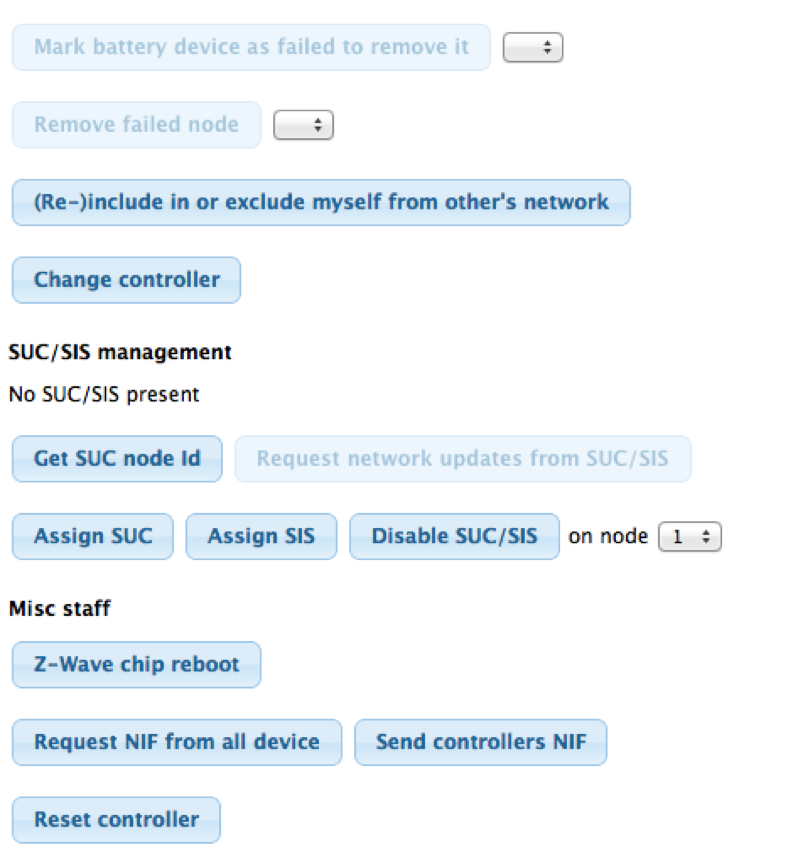
\includegraphics[scale=0.8]{pics/network2.png}
\caption{Demo UI Dialog for Networking functions - experts functions}
\label{c1:network2} 
\end{center} \end{figure}


The controller change function allows to handover the primary function to a different 
controller in the network. The function works like a normal inclusion 
function but will hand over the primary privilege to the new controller after inclusion. 
Z-Way will become a secondary controller of the network. This function may be needed 
during installation of larger networks based on remote controls only where Z-Way is 
solely used to do a convenient network 
setup and the primary function is finally handed over to one of the remote controls.

This function is implemented with the function class {\bf ControllerChange()}. Please 
refer to the chapter \ref{FunctionClasses} for details on how to use this function.

\subsection {SUC/SIS Management}

This interface allows controlling the SUC/SIS function for the Z-Wave network. All 
these functions are almost obsolete and only needed for certain enhanced configurations 
of the Z-Wave network. Unless you really know what you do - don't use these functions!

The following Function Classes are mapped to the demo user interface  functions 
for SUC/SIS manipulation:
\begin{itemize}
\item GetSUCNodeId - get the SUC Node ID from the network
\item EnableSUC - enables the SUC function in Z-Way, this is done by default if the transceiver firmware used supports SUC
\item SetSUCNodeId - assign SUC function to a node in the network that is capable of running there SUC function.
\item SendSUCNodeId - inform a different node about the node ID of a SUC in the system
\end{itemize}


 
\subsection{Routing Table}


\begin{figure} 
\begin{center}
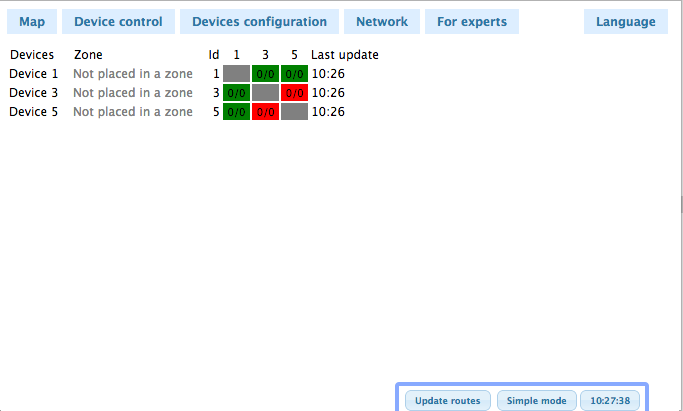
\includegraphics[scale=0.5]{pics/routingtable.png}
\caption{Demo UI dialog for Routing Table}
\label{c2:demorouting} 
\end{center} \end{figure}

The routing table of the Z-Wave network is shown in the tab network as well. It indicates how two devices of the Z-Wave network can communicate with each other. 
If two devices are in direct range (they can communicate without the help of any other node) the cross point of the two devices in the table is marked as dark green. 
The color light green indicates that the two nodes are not in direct range but have more than one alternating routes with one node between. This is still considered 
as a stable connection.
The yellow color indicates that there are less than two “one-hop” routes available between the two nodes. However there may be more routes but with more nodes
 between and therefore considered as less stable.

A red indicator shows that there are no good short connections between the two nodes. This does not mean that they are unable to communicate with each other 
 but any route with more than 2 routers between Z-Way is considering as not reliable, even taking into account that Z-Wave supports routes with up to four devices 
 between. Grey cells indicate the connection to the own Node ID. 

The general rule of thumb is: 'The greener the better'.
 
The table lists all nodes on the y-axis and the neighborhood information on the x-axis. On the right hand side of the table a timestamp shows when the neighborhood
 information for a given node was reported.   

In theory the table should be totally symmetric, however different times of the neighborhood detection may result in different neighborhood information of the 
two devices involved.
 
The neighbor information of the controller works with an exception. The Z-Wave implementation used in current Z-Wave transceiver does not allow requesting an 
update of the neighbor list for the controller itself. The neighborhood information displayed for the controller is therefore simply wrong.

Battery powered devices will report their neighbors when woken up and report their mains powered neighbor correctly. However mains powered devices will report 
battery-powered devices as neighbors only when routes are updated twice. This is less critical because battery powered devices can’t be used as routers and are 
therefore not relevant for calculating route between two nodes anyway. 
 
The context menu command 'Network Reorganization' allows re-detecting all neighborhood information (battery powered devices will report after their next wakeup!) 
Please refer to the manual section 'Network Stability' for further information about the use of this function.

The routing table is stored in the Z-Wave transceiver and can be read using the function class {\bf  GetRoutingTableLine(node id)} for a given node ID. The function 
{\bf RequestNodeNeighbourUpdate(nodeid)} will cause a certain node Id to redirect its
 wireless neighbors. It makes sense to call the GetRoutingTable function right 
after successful callback of the RequestNodeNeighbourUpdate function. 

 